
\documentclass{article} % For LaTeX2e
\usepackage{iclr2027_conference,times}

% Optional math commands from https://github.com/goodfeli/dlbook_notation.
\input{math_commands.tex}

\usepackage{hyperref}
\usepackage{url}

\usepackage{algorithm}
\usepackage{algorithmic}

\usepackage{booktabs}
\usepackage{graphicx}
\usepackage{amsmath,amssymb}
\usepackage{threeparttable}


\title{Counterfactual Plasticity: Risk-Aware Selection of Model Updates Before Execution}

% Authors must not appear in the submitted version. They should be hidden
% as long as the \iclrfinalcopy macro remains commented out below.
% Non-anonymous submissions will be rejected without review.

\author{Anonymous Authors}

% The \author macro works with any number of authors. There are two commands
% used to separate the names and addresses of multiple authors: \And and \AND.
%
% Using \And between authors leaves it to \LaTeX{} to determine where to break
% the lines. Using \AND forces a linebreak at that point. So, if \LaTeX{}
% puts 3 of 4 authors names on the first line, and the last on the second
% line, try using \AND instead of \And before the third author name.

%\iclrfinalcopy % Uncomment for camera-ready version, but NOT for submission.
\begin{document}


\maketitle

\begin{abstract}
Post-training updates can successfully teach a model new information while
simultaneously damaging previously reliable behavior.
When multiple candidate updates are available, this raises a natural decision
problem: can we predict their consequences before execution and choose the
update that provides useful acquisition with lower collateral risk?

We formulate this problem as \emph{counterfactual update selection} and
introduce \textbf{Counterfactual Plasticity}, a risk-aware framework that uses
pre-update fingerprints to forecast candidate acquisition gain, collateral
damage, and damage uncertainty.
Rather than relying only on point predictions, the method calibrates the
induced update-selection rule using held-out split conformal risk control,
selecting the highest-gain admissible update or abstaining when no candidate is
sufficiently supported.

Controlled experiments reveal a pronounced asymmetry between acquisition and
damage forecasting: acquisition is comparatively predictable, whereas damage
is more brittle and particularly vulnerable to structural changes in the
candidate action space.
In benign regimes, an uncalibrated selector is already nearly harmless;
under structurally ambiguous update menus, however, naive forecast-based
selection can fail sharply.

We therefore evaluate the final method prospectively on fresh factual-editing
data using TinyLlama and Gemma under frozen one-shot protocols.
On held-out test edits, Counterfactual Plasticity reduces harmful-update rates
from $24.4\%$ to $7.8\%$ on TinyLlama and from $23.3\%$ to $8.9\%$ on Gemma,
with paired $95\%$ confidence intervals for both reductions entirely below
zero.
The resulting policies remain adaptive rather than collapsing to a single
conservative intervention.
These results suggest that model updating can be improved by reasoning about
multiple possible parameter-space futures before deciding which update should
become real.
\end{abstract}

\section{Introduction}
\label{sec:introduction}

Modern language models are increasingly expected to change after pretraining.
Factual correction, continual learning, personalization, domain adaptation,
and model editing all modify a model that already possesses useful
capabilities. Yet acquiring new information can also perturb unrelated
knowledge or previously reliable behavior. This creates a basic plasticity
problem: \emph{how should a model be updated when several plausible updates
differ in both benefit and collateral effects?}

Most update procedures are evaluated retrospectively: an intervention is
applied, target behavior is measured, and collateral degradation is assessed
afterward. But the same intended change can often be implemented through
several candidate interventions---for example, different learning rates,
optimization durations, parameter scopes, or layer locations---with different
acquisition--damage trade-offs. We therefore ask whether these consequences
can be estimated \emph{before} execution and used to decide which candidate,
if any, should become real.

We call this problem \emph{counterfactual update selection}. Given a model
state, a new experience, and a finite candidate set, the goal is to forecast
each candidate's acquisition gain and collateral damage from pre-update
information, then select one candidate or abstain. This treats updating as a
decision over possible parameter-space futures rather than as a predetermined
optimization step.

Our controlled experiments reveal a recurring asymmetry: acquisition is
comparatively easy to forecast, whereas damage is more brittle across model
families, distributional regimes, and candidate action spaces. Ensemble
uncertainty is informative in several settings but can fail under structural
action-space shift. In a heterogeneous controlled stress test, for example,
the uncalibrated selector is harmful on 51.5\% of episodes and frozen CP
reduces this to 38.5\% without eliminating the failure. This motivates
calibrating the \emph{decision rule} rather than trusting point forecasts
alone, while also delimiting the scope of that calibration.

We introduce \textbf{Counterfactual Plasticity} (CP), a risk-aware decision
layer over a finite candidate-update menu. CP constructs a pre-update
fingerprint for each candidate, forecasts acquisition gain, collateral damage,
and damage uncertainty, excludes candidates inconsistent with a calibrated
damage criterion, and selects the highest-predicted-gain admissible candidate
or abstains. In the final external evaluation, the conservatism of this rule
is selected with split conformal risk control on held-out calibration edits,
with the test set untouched.

We evaluate CP under a frozen E1 factual-editing protocol on TinyLlama and
Gemma with disjoint training, calibration, and one-shot test splits. On 90
held-out edits per model, CP reduces the harmful-decision rate of the
uncalibrated ensemble selector (B1) from 24.4\% to 7.8\% on TinyLlama and from
23.3\% to 8.9\% on Gemma. The paired reductions are 16.7 and 14.4 percentage
points, with both 95\% confidence intervals entirely below zero. The utility
cost differs by model: TinyLlama trades acquisition for lower risk and
abstains on 17/90 edits, whereas Gemma retains essentially unchanged
acquisition with no test abstentions. CP remains adaptive, selecting all six
candidate procedures on TinyLlama and five of six on Gemma.

The contribution is therefore not a new mechanism for constructing a
particular edit, but a decision layer that forecasts and selects among
\emph{complete candidate parameter-update procedures before execution}. This
distinguishes CP from methods that adapt how a single editing mechanism is
internally constructed.

This distinction fixes both the action and the timing of the decision. An
adaptive editor may use properties of an edit to choose an internal layer,
parameter subset, or edit-specific construction within its own mechanism. CP
is agnostic to how a candidate is constructed: such adaptive editors can be
members of $\mathcal C$, alongside ordinary optimization procedures. CP instead
decides, from information available before execution, which complete procedure
to instantiate on the current model state, or whether none is adequately
supported. Likewise, CP is not a model-editing algorithm that claims a better
post-edit representation; its object is the pre-execution policy over a fixed
menu of possible updates. This separation permits the risk--utility decision
to be studied without attributing improvements to a particular editing
mechanism.

Our contributions are:
\begin{itemize}
    \item We formulate \textbf{counterfactual update selection}: choosing among
    candidate parameter updates from pre-update information while balancing
    acquisition gain against collateral damage.

    \item We characterize an empirical forecasting asymmetry in which
    acquisition is comparatively predictable while damage is more brittle,
    including a structural action-space regime where uncertainty and frozen
    risk calibration fail to transfer reliably.

    \item We introduce \textbf{Counterfactual Plasticity}, combining pre-update
    forecasting, ensemble uncertainty, decision-level calibration, and
    abstention to select among complete candidate updates.

    \item We provide frozen external factual-editing evaluations on TinyLlama
    and Gemma, where CP substantially reduces harmful-decision rates while
    retaining adaptive update selection.
\end{itemize}

These results are not a universal safety guarantee. The calibrated procedure
is tied to its candidate-action distribution and stated evaluation
assumptions, and arbitrary distribution shift can invalidate the conditions
under which its risk calibration is meaningful.

\section{Counterfactual Update Selection}
\label{sec:problem}

For model parameters $\theta$, a new experience $x$, and a finite menu of
update procedures $\mathcal{C}=\{c_1,\ldots,c_K\}$, candidate $c$ produces
$\theta'_c=U(\theta,x;c)$. Candidates can differ in optimization strength,
duration, parameter scope, or layer location. We must select one candidate
before executing any of them.

Let $\ell_x$ be target loss and let $\mathcal P=\{p_1,\ldots,p_M\}$ be a
protected set. The realized acquisition gain and collateral damage are
\[
G(c)=\ell_x(\theta)-\ell_x(\theta'_c),\qquad
D(c)=\frac1M\sum_{j=1}^M[\ell_{p_j}(\theta'_c)-\ell_{p_j}(\theta)].
\]
Larger $G$ is better and positive $D$ is degradation. With prospectively fixed
damage budget $\tau$, a selected update is harmful when
$H(c)=\mathbb I[D(c)>\tau]$. These outcomes are observable only after the
candidate is run.

CP instead forms a pre-execution fingerprint $\phi(\theta,x,c)$ and predicts
$(\widehat G_c,\widehat D_c,\widehat U_c)$ for every $c\in\mathcal C$.
The resulting alternatives are \emph{counterfactual updates}. $\phi$ contains
only pre-update information; realized gains, damages, harm labels, and
post-execution statistics are unavailable at decision time. Thus the task is
not prediction error alone: a forecaster can err most on the high-gain
candidates a selector prefers. We seek a policy
\[
\pi:\{\phi(\theta,x,c)\}_{c\in\mathcal C}\to\mathcal C\cup\{\bot\}
\]
that obtains acquisition while controlling $\mathbb E[H(\pi(x))]$;
abstention $\bot$ executes no update and has zero harmful-update loss.
Forecasting, risk estimation, and selecting the highest-utility admissible
candidate are consequently distinct problems. The diagnostic oracle and full
feature specification are given in Appendix~\ref{app:method_details}.

The protected set defines the operational meaning of collateral damage rather
than an exhaustive notion of preservation. In particular, $D(c)$ averages loss
changes over the prespecified protected items, and $H(c)$ records whether that
average exceeds the fixed budget. The policy is evaluated once per requested
experience, not once per candidate: candidates that are considered but not
executed have no realized contribution to the decision loss. This is why
candidate-level forecast quality alone is insufficient for the stated
decision problem, and why a safe-looking candidate menu can still yield a
risky selector when its ranking favors systematically underestimated updates.

\section{Counterfactual Plasticity}
\label{sec:method}

CP uses pre-update fingerprints to forecast candidate gain and damage, then
calibrates the \emph{decision induced by these forecasts}, not a simultaneous
guarantee for every candidate prediction. Let $\mu_G(c)$ rank candidates and
let $\mu_D(c)$ and ensemble disagreement $\sigma_D(c)$ be the damage forecast
and empirical uncertainty signal, respectively. (Architecture, features, and
the interpretation limits of disagreement are in
Appendix~\ref{app:method_details}.) For conservatism $\lambda\geq0$, CP admits
\[
\mathcal A_\lambda(x)=\{c\in\mathcal C:
\mu_D(c)+\lambda\sigma_D(c)\leq\tau\},\qquad
\pi_\lambda(x)=\arg\max_{c\in\mathcal A_\lambda(x)}\mu_G(c),
\]
and abstains when $\mathcal A_\lambda(x)=\varnothing$. This separates utility
ranking from damage admissibility and makes uncertainty operational rather
than a claimed posterior probability of harm.

\paragraph{Decision-level split CRC.}
For an edit $i$, the raw loss is
\[
L_i(\lambda)=\mathbb I[D_i(\pi_\lambda(x_i))>\tau]
\]
when CP selects an update and $0$ on abstention. Candidate switching means
that raw policy loss need not be monotone along a scalar $\lambda$ path. We
therefore calibrate an all-supersets monotone closure over \emph{forbidden
sets}, not scalar-path shorthand. For $F\subseteq\mathcal C$, let $\pi(F)$
choose the highest-predicted-gain member of $\mathcal C\setminus F$ (or
abstain if none remains), and define
\[
\ell_0(y,F)=\mathbb I[D(y,\pi(F))>\tau]\quad(=0\text{ on abstention}),
\qquad
\widetilde\ell(y,F)=\max_{F'\supseteq F}\ell_0(y,F').
\]
Thus, for $F_1\subseteq F_2$, $\widetilde\ell(y,F_1)\geq
\widetilde\ell(y,F_2)$, while $\ell_0(y,F)\leq\widetilde\ell(y,F)$.
For numerical $\lambda$, $F_\lambda(x)=\{c:\mu_D(x,c)+
\lambda\sigma_D(x,c)>\tau\}$. This exact all-supersets closure is essential;
it is not defined by $\sup_{\lambda'\geq\lambda}L_i(\lambda')$.

In E1 we enumerate all $2^6=64$ forbidden sets for every calibration edit and
use the ordered family
\[
\Lambda_{\rm E1}=\{0,0.25,0.50,\ldots,15.00\},\ \texttt{FORCED\_ABSTAIN},
\]
with 61 numerical $\lambda$ values. The terminal state forbids all candidates,
executes no update, and has zero raw and closure loss. With 90 disjoint
calibration edits and $\alpha=.10$, split CRC chooses the first eligible state
using exactly
\[
\frac{1+\sum_{i=1}^{90}\widetilde\ell(y_i,F_\lambda(x_i))}{91}\leq .10.
\]
It therefore accepts at most eight closure losses; \texttt{FORCED\_ABSTAIN}
ensures selection is defined if no numerical value is eligible. Forecast
training, calibration, and final testing are disjoint. This E1 construction is
distinct from the controlled v0.1 10-fold CV-CRC procedure.

\paragraph{Scope.} Conditional on fixed E1 training data and a fixed pipeline
(finite candidate set, features, forecasters, grid, deterministic policy, and
damage/reset scoring rule), split CRC controls expected average
harmful-update loss for a future edit exchangeable with the 90 calibration
edits. The closure bound transfers this statement to the raw selected-update
loss, with zero loss on abstention. It is not a per-edit, universal,
realized-rate confidence, or online-deployment guarantee. It also depends on
the finite candidate space and on offline calibration data containing every
counterfactual candidate outcome. Appendix~\ref{app:method_details} gives the
full construction, tie-breaking, proof details, and inference pseudocode.

Two details are worth making explicit. First, the guarantee concerns the
random loss of the selected policy on a future exchangeable edit; it is not a
claim that at most $\alpha$ of the 90 realized test decisions must be harmful.
Finite test samples can fluctuate around their expectation. Second, abstention
is part of the loss definition, not evidence that an unexecuted candidate was
safe: it means that the policy commits no parameter update and therefore
incurs zero harmful-update loss under this metric. Its practical cost is
foregone acquisition, which is reported separately. Thus split CRC calibrates
one precisely specified harm--abstention decision, rather than certifying all
candidate predictions or all dimensions of model behavior.

\section{When Does Risk-Aware Update Selection Matter?}
\label{sec:controlled}

We first ask when risk-aware selection is necessary rather than merely
conservative. In controlled GPT-2 update episodes spanning facts, symbols,
rules, and arithmetic, every candidate is executed from the same reset
checkpoint and harm is defined as $D>\tau$ with $\tau=0.01$. Forecasts use only
pre-update fingerprints. These experiments are mechanistic development
diagnostics; the controlled v0.1 policy uses a separate 10-fold CV-CRC
procedure and does not inherit the E1 split-CRC guarantee.

\paragraph{Forecasting asymmetry.}
Acquisition is consistently easier to predict than collateral damage. In the
original menu, ensemble damage uncertainty strongly tracks absolute damage
error (Spearman $\rho\approx0.87$ on calibration episodes and $0.85$ on
held-out episodes), showing that disagreement can be useful even when damage
point estimates are imperfect. The decision problem is nevertheless harder
than average prediction error: a selector can preferentially choose the
high-gain candidates whose damage is most underestimated.

\paragraph{Benign menus.}
Risk calibration adds little when the action space is already safe. Under the
original eight-candidate menu, the point-estimate selector achieves mean
$G=9.717$ with one harm in 30 episodes, while B1 achieves $G=9.702$ with zero
harms. Harder experiences with the same menu produce 0/400 B1 harms, and a
densified update-strength menu produces only 1/400. Thus, neither harder
experiences nor the mere presence of harmful candidates is sufficient; harmful
updates must also be competitive under the forecasted utility landscape.

\paragraph{Structural ambiguity.}
We therefore introduce a heterogeneous menu varying learning rate, duration,
parameter scope, layer location, and width. High-gain full-scope candidates
now compete with safer localized updates, creating genuine risk pressure.
Frozen B1 is harmful on $206/400=51.5\%$ of episodes, while frozen CP reduces
this to $154/400=38.5\%$. All B1 harms are full-scope selections. Crucially,
within that high-risk subspace the uncertainty--error association collapses to
$\rho\approx0.07$, and harmful full-scope outcomes are systematically
underpredicted. Retraining on this regime sharply reduces harm, indicating a
transport failure in damage forecasting rather than an inherent inability to
separate every risky update.

The S2 result also sharpens what ``structural'' means here. The issue is not
simply that a test episode is more difficult, nor that a menu contains more
candidates. The heterogeneous menu introduces qualitatively different
full-scope actions whose high predicted gain makes them competitive in the
selector's ranking. Within precisely that region, damage is underpredicted and
disagreement ceases to identify the largest errors. Frozen calibration can
then exclude candidates according to a signal whose ordering no longer tracks
the relevant failure mode. The partial reduction from 51.5\% to 38.5\% is
therefore descriptive evidence of limited transfer, not evidence that CP
solves the shifted regime; the improvement after retraining instead points to
the need for calibration data representative of the available action space.

Figure~\ref{fig:controlled_regime_summary} summarizes the key contrast. The
negative cases are important: CP is not automatically beneficial when B1 is
already benign, and frozen calibration need not transfer across a structurally
changed action space. These lessons motivate the E0/E1 design below.

\begin{figure*}[t]
    \centering
    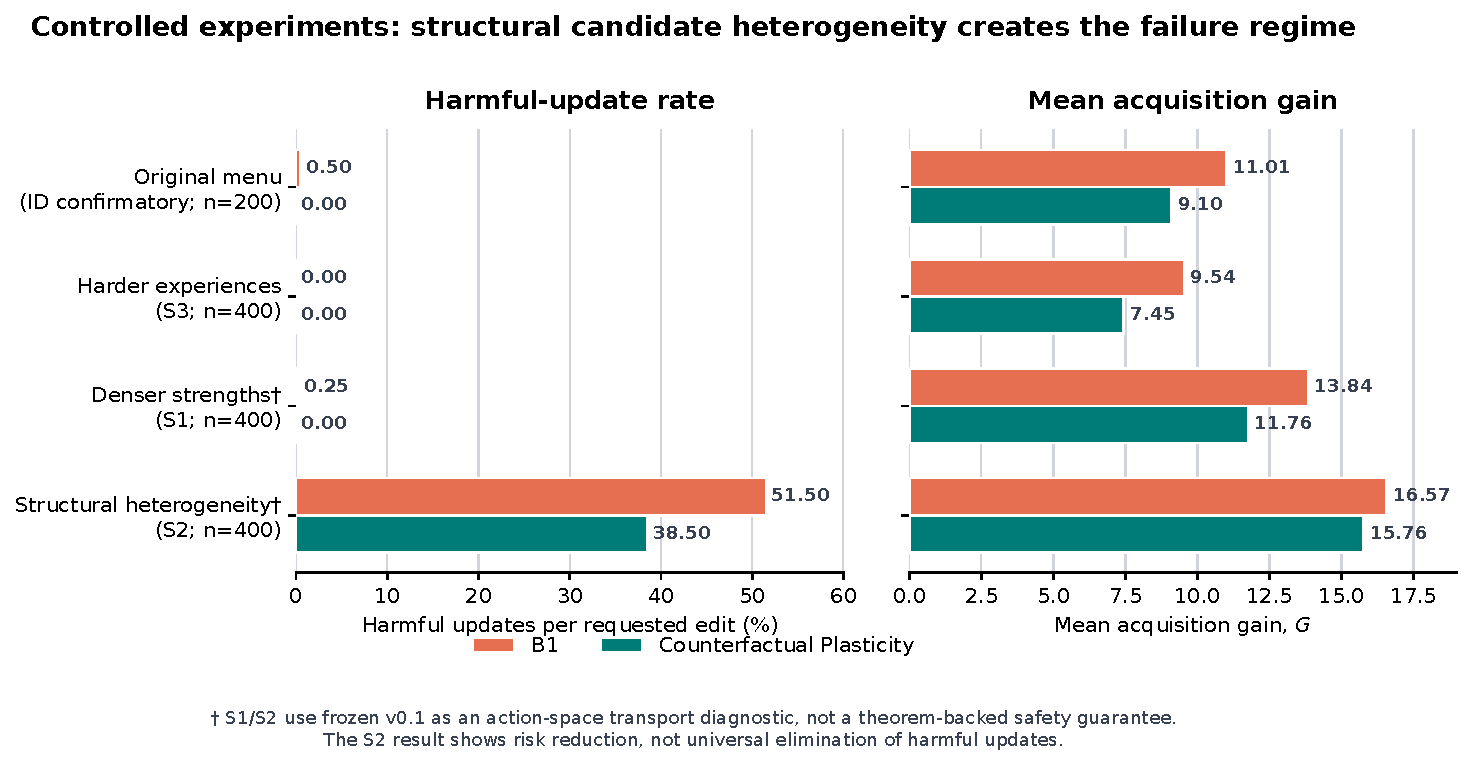
\includegraphics[width=\textwidth]{paper2_controlled_regime_summary.pdf}
    \caption{\textbf{Controlled regime summary.} Frozen B1 and CP are nearly
    harmless in the original menu, harder-experience S3, and denser-strength S1
    settings. Structural candidate heterogeneity in S2 creates substantial
    harmful-update pressure (51.5\% for B1); frozen CP reduces this to 38.5\%
    but does not eliminate it. S1/S2 are transport diagnostics rather than
    theorem-backed E1 risk guarantees.}
    \label{fig:controlled_regime_summary}
\end{figure*}

Additional B0/B1/B2 progression, S1/S3 diagnostics, and retraining analyses are
reported in Appendix~\ref{app:controlled_details}.

\section{Prospective External Factual Editing}
\label{sec:external}

We next evaluate whether such decision pressure appears in factual editing.
The external study separates a descriptive development screen (E0) from a
fresh frozen confirmatory evaluation (E1). E0 evaluates Qwen, TinyLlama, and
Gemma on 60 edits under six fixed candidate procedures and 120 protected
facts. Qwen is nearly benign, whereas TinyLlama and Gemma exhibit substantial
gain--damage trade-offs; those two regimes are therefore carried forward to
E1. This is development-stage model/regime selection, not a prospective E0
claim, and no E0 example is reused in E1.

The E0-to-E1 separation is intentional. E0 asks whether the fixed menu creates
enough decision pressure to make a risk--utility policy informative: in a
nearly benign regime, reducing an already rare harm rate would be difficult to
interpret and could be achieved by needless conservatism. TinyLlama and Gemma
showed nontrivial trade-offs under the development screen, so they were chosen
as the two frozen evaluation regimes. E1 then uses new edits, new protected
items, disjoint forecast-training and calibration splits, and a locked test
split. Consequently, E0 supports the choice of where to evaluate rather than
the final risk claim, which rests on the separately frozen E1 protocol.

\subsection{Frozen E1 protocol}
\label{sec:e1_protocol}

For each model, E1 uses 360 fresh CounterFact edits and 180 fresh protected
items, with the same identities across models but independent forecasting and
calibration. Edits are grouped into 180 training, 90 calibration, and 90
locked one-shot test edits, with all six candidates for an edit kept in the
same split. Before test outcomes are observed, we freeze the data manifests,
model/tokenizer revisions, candidate mappings, feature schema, forecasters,
seeds, baselines, $\tau=0.01$, split-CRC target $\alpha=0.10$, tie-breaking,
abstention, and evaluation rules.

Split-CRC selects $\widehat\lambda=2.25$ for TinyLlama and $3.00$ for Gemma.
The 90-edit calibration criterion permits at most eight closure losses:
TinyLlama attains $9/91=0.0989$ regularized risk with eight closure losses,
while Gemma attains $7/91=0.0769$ with six. The exact forbidden-set
construction and its expected-risk scope are given in
Section~\ref{sec:method} and Appendix~\ref{app:method_details}.

Each edit--candidate pair is independently restored, fingerprinted, executed,
and evaluated against all 180 protected items. The primary comparator is B1,
which uses the same six-candidate action space and forecasting machinery as CP
but without calibrated decision-level exclusion. Harm is measured per
requested edit, with abstention assigned zero harmful-decision loss.

\subsection{Locked E1 results}
\label{sec:e1_main_results}

Table~\ref{tab:e1-primary-results} gives the frozen test results.

% Requires: \usepackage{booktabs,threeparttable}
% First E1 table only. The diagnostic-oracle table is in a separate file.

\begin{table*}[ht]
\centering
\caption{\textbf{Locked E1 protocol, calibration, and primary external factual-editing results.}
Each model uses 180 training edits, 90 calibration edits, and 90 locked test edits; the protected set has 180 items and the action space has six frozen update procedures. Harm is $1[D>0.01]$. Split CRC targets $\alpha=0.10$. Harm rates are per requested edit (abstentions contribute zero harm); conditional CP harm is reported among executed updates.}
\label{tab:e1-primary-results}

\small
\begin{threeparttable}
\textit{Protocol and calibration}\\[-2pt]
\begin{tabular}{lccccc}
\toprule
Model & Train / Cal. / Test & Protected & Candidates & $\lambda$ & Closure losses; $R_{\mathrm{CRC}}$ \\
\midrule
TinyLlama & 180 / 90 / 90 & 180 & 6 & 2.25 & $8/90$; $9/91=0.098901$ \\
Gemma     & 180 / 90 / 90 & 180 & 6 & 3.00 & $6/90$; $7/91=0.076923$ \\
\bottomrule
\end{tabular}

\textit{Locked test results}\\[-2pt]
\begin{tabular}{lcccccc}
\toprule
Model & \multicolumn{2}{c}{B1} & \multicolumn{4}{c}{Counterfactual Plasticity} \\
\cmidrule(lr){2-3}\cmidrule(l){4-7}
& $G$ & Harm & $G$ & Harm & Harm|exec. & Abstain \\
\midrule
TinyLlama & 7.294038 & 24.44\% & 6.155598 & 7.78\% & 9.59\% & 18.89\% \\
Gemma     & 21.311913 & 23.33\% & 21.307810 & 8.89\% & 8.89\% & 0\% \\
\bottomrule
\end{tabular}

\begin{tablenotes}[flushleft]\footnotesize
\item \textit{Denominator.} The primary harm denominator is all 90 requested test edits. The conditional column uses only non-abstained edits and is supplementary.
\end{tablenotes}
\end{threeparttable}
\end{table*}


CP substantially reduces harmful decisions relative to B1 on both models. On
TinyLlama, harm falls from $22/90=24.4\%$ to $7/90=7.8\%$, a paired reduction
of $16.67$ percentage points (95\% CI $[-24.44,-8.89]$). On Gemma, harm falls
from $21/90=23.3\%$ to $8/90=8.9\%$, a reduction of $14.44$ points (95\% CI
$[-22.22,-7.78]$).

The utility cost is model dependent. TinyLlama loses $1.1384$ mean acquisition
relative to B1 (95\% CI $[-1.7186,-0.6274]$) and abstains on 17/90 edits;
among executed updates, harm is $7/73=9.6\%$. Gemma changes acquisition by
only $-0.00410$ (95\% CI $[-0.00621,-0.00238]$) and never abstains. CP does
not collapse to a static rule: it uses all six candidates on TinyLlama and five
of six on Gemma.

The contrast between models is informative rather than a discrepancy to be
averaged away. For TinyLlama, CP's lower harm rate is accompanied by fewer
executed opportunities and lower mean acquisition, so its 17 abstentions make
the risk reduction visibly costly under this utility measure. For Gemma, the
same decision framework reduces observed harm while retaining nearly the same
mean acquisition and executing every test edit. These outcomes do not imply
that one model is intrinsically safer, nor that a single operating point is
optimal for all deployments. They show that the value of calibrated exclusion
depends on how candidate gain, damage, and forecast uncertainty jointly align
within a model-specific regime; reporting harm without acquisition and
abstention would obscure that distinction.

Figure~\ref{fig:e1_primary_risk_utility} summarizes the joint risk--utility
trade-off.

\begin{figure*}[t]
    \centering
    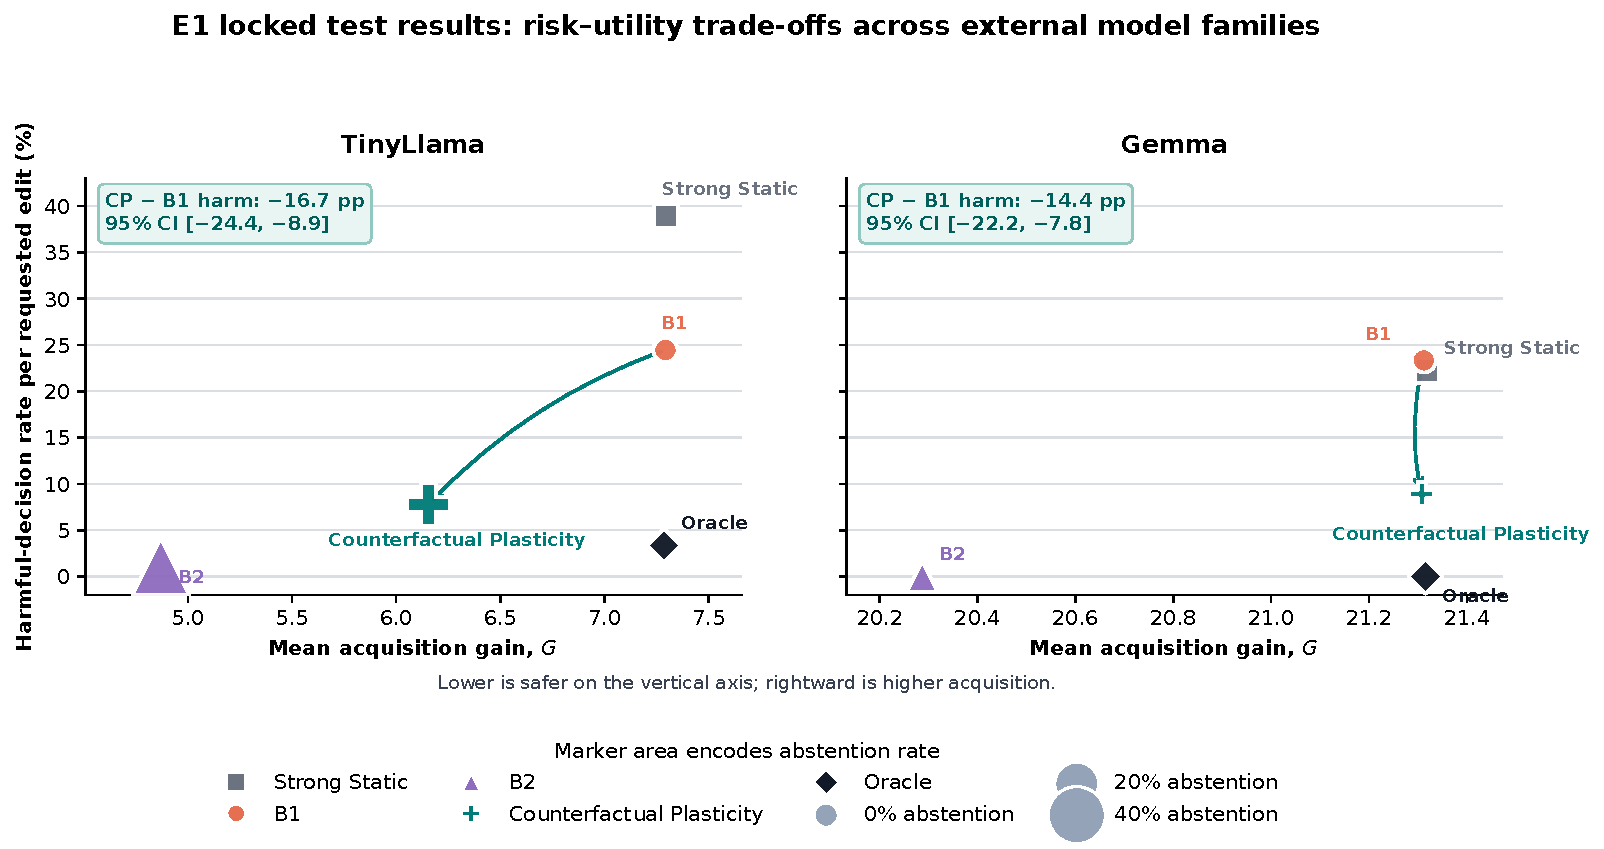
\includegraphics[width=0.93\textwidth]{paper2_e1_primary_risk_utility_figure.pdf}
    \caption{\textbf{Locked E1 risk--utility trade-offs.} Across 90 held-out
    edits per model, CP substantially reduces harmful decisions relative to B1.
    Marker area encodes abstention. The annotated CP--B1 harm-rate differences
    use the preregistered paired bootstrap intervals. B2 is shown only as a
    descriptive prediction-level conformal baseline; no CP--B2 inferential
    comparison was preregistered.}
    \label{fig:e1_primary_risk_utility}
\end{figure*}

The descriptive B2 baseline is more conservative: on TinyLlama it yields
1/90 harms with 35 abstentions and mean $G=4.870$, while on Gemma it yields
0/90 harms with five abstentions and mean $G=20.287$. CP attains higher mean
$G$ and fewer abstentions in both cases, but we make no inferential CP--B2
superiority claim. The diagnostic oracle also need not be harm-free: when no
candidate satisfies $D\leq\tau$, it selects the minimum-damage candidate rather
than abstaining, which explains three TinyLlama oracle harms.

E1 also reproduces the forecasting asymmetry. Gain $R^2$ is $0.994$ on
TinyLlama and $0.992$ on Gemma, versus damage $R^2$ of $0.485$ and $0.656$.
Damage uncertainty remains positively associated with absolute damage error
($\rho=0.557$ and $0.459$, respectively), unlike the full-scope S2 failure.
Extended E0 details, candidate-selection distributions, B2 table, oracle
statistics, and forecasting diagnostics are in
Appendix~\ref{app:external_details}.

\section{Analysis and Ablations}
\label{sec:analysis}

The primary matched comparison is CP versus B1 because both share the same
forecasters and six-candidate action space; the difference is decision-level
calibration. Two diagnostics clarify the result.

\paragraph{Decision-level versus prediction-level protection.}
B2 conformalizes candidate damage predictions before selection and is more
conservative than CP. On TinyLlama, B2 yields 1/90 harms, 35 abstentions, and
mean $G=4.870$, versus 7.8\% harm, 17 abstentions, and $G=6.156$ for CP. On
Gemma, B2 yields 0/90 harms, five abstentions, and $G=20.287$, versus 8.9\%
harm, no abstentions, and $G=21.308$ for CP. These point estimates illustrate
the utility/coverage cost of prediction-level protection, but no paired
CP--B2 inference was preregistered, so we make no superiority claim.

\paragraph{Forecasting and uncertainty.}
E1 reproduces the controlled asymmetry. Gain $R^2$ is $0.994$ on TinyLlama and
$0.992$ on Gemma, versus damage $R^2$ of $0.485$ and $0.656$. Candidate-level
damage uncertainty remains positively associated with absolute damage error
($\rho=0.557$ and $0.459$), but the S2 full-scope result ($\rho\approx0.07$)
shows that this relation can collapse exactly where structural risk
concentrates. Ensemble disagreement is therefore a useful empirical signal,
not a universal certificate.

This asymmetry also identifies a failure boundary for forecasting-based
selection. High gain $R^2$ does not by itself validate a selector, because the
policy can be sensitive to a small subset of high-gain candidates whose damage
is badly underestimated. Conversely, a positive aggregate association between
$\sigma_D$ and damage error does not ensure that the association holds in the
subpopulation selected by the policy. The S2 full-scope analysis provides the
counterexample: uncertainty can look useful overall while losing resolution
where risk is concentrated. Forecast diagnostics should therefore be read as
evidence about a fixed regime, with action-space composition and selected
subgroups treated as part of the deployment distribution.

These diagnostics reinforce the method's intended scope: calibration helps
when naive selection faces real risk and the calibration regime remains
relevant, but it cannot rescue arbitrary action-space shift. Extended tables,
selection distributions, oracle statistics, and forecasting plots are in
Appendix~\ref{app:external_details}.

\section{Related Work}
\label{sec:related_work}

Model editing modifies pretrained models while trying to preserve unrelated
behavior. Representative methods include MEND \citep{mitchell2022mend}, ROME
\citep{meng2022rome}, MEMIT \citep{meng2023memit}, and SERAC
\citep{mitchell2022serac}. Recent adaptive editors choose layers or internal
components per edit, including FiDAL, CAKE, and HiEdit. CP addresses a
complementary decision: it treats a \emph{complete candidate update procedure}
as the action and forecasts which candidate should be executed before any
candidate outcome is observed.

Continual-learning work studies plasticity--stability trade-offs across
sequences of tasks, while influence-style methods and update-effect predictors
estimate how training examples or parameter changes affect model behavior
\citep{koh2017understanding}. CP differs by coupling pre-update consequence
forecasting to an explicit finite-action selection rule.

Ensemble methods provide useful epistemic diagnostics
\citep{lakshminarayanan2017deep}, but CP does not interpret ensemble
disagreement as a calibrated probability of harm. Instead, conformal risk
control \citep{angelopoulos2024conformal} calibrates the bounded harmful-update
loss induced by the final decision. Candidate switching makes raw loss
non-monotone in scalar conservatism, motivating the all-supersets forbidden-set
closure in Section~\ref{sec:method}. The resulting statement applies only
under the fixed-pipeline and exchangeability assumptions already stated; it is
not a universal safety guarantee.

\section{Limitations and Discussion}
\label{sec:limitations}

CP reduces harmful selections in E1, but its validity is conditional on the
specified candidate family and calibration regime. Split CRC controls expected
average harmful-update loss for future edits exchangeable with calibration
examples under a fixed pipeline; it is not a per-edit, realized-rate,
online-deployment, or arbitrary-shift guarantee. The controlled S2 experiment
shows why: structural action-space change can produce systematic damage
underestimation and weaken the uncertainty signal exactly where risk
concentrates.

Damage forecasting remains the central bottleneck. Acquisition is
comparatively predictable, whereas collateral damage varies with model family,
scope, and candidate structure. Conservative policies can always reduce harm
by excluding powerful interventions, so low risk must be interpreted jointly
with utility and abstention. This trade-off is visible on TinyLlama (17/90 CP
abstentions) but not on Gemma (0/90).

The method also inherits limitations from its finite action menu and protected
set. If all candidates are harmful or ineffective, selection cannot recover a
good intervention; and preserving 180 protected factual items does not imply
preservation of all knowledge, reasoning, style, or safety-relevant behavior.
Our external evidence is limited to factual editing on two E1-selected model
regimes, so transfer to continual learning, preference optimization,
personalization, or safety interventions remains open. Finally, offline
training/calibration requires evaluating every candidate outcome and protected
loss vector; deployment executes only the selected candidate, but fingerprint
extraction still incurs gradient cost.

These limitations also explain the controlled negative results. Calibration is
most useful when multiple candidates genuinely compete and naive selection
creates material risk; in benign menus it may only sacrifice utility, while
under strong action-space shift it may fail to transfer. CP should therefore be
viewed as a calibrated decision layer for a specified intervention regime, not
as a universal model-update safety mechanism.

An immediate implication is that extending CP to a new updater, parameter
scope, or protected-behavior definition requires re-establishing the pipeline
rather than reusing a numerical conservatism value by default. The candidate
menu is not merely an implementation detail: it determines which
counterfactuals are ranked, which forbidden sets are calibrated, and the
abstention alternatives available to the policy. More comprehensive protected
evaluations may improve the substantive meaning of damage, but they can also
change the calibration target and cost. These are empirical design choices,
not consequences of the split-CRC statement alone.

\section{Conclusion}
\label{sec:conclusion}

We introduced \textbf{Counterfactual Plasticity}, which frames post-training adaptation as a calibrated decision among candidate updates before any update is committed. Using pre-update fingerprints, it forecasts acquisition utility and collateral risk, accounts for uncertainty in the latter, and calibrates update selection against harmful-update risk.

Controlled experiments show why this distinction matters: acquisition utility is easier to forecast than collateral risk, and naive forecast-based selection can fail when high-gain, high-damage interventions compete. Prospective frozen-protocol factual editing on TinyLlama and Gemma then shows that Counterfactual Plasticity reduces harmful-update rates from $24.4\%$ to $7.8\%$ and from $23.3\%$ to $8.9\%$, respectively, while retaining adaptive candidate selection.

The method does not guarantee safety under distribution or action-space shift. Its broader contribution is a decision framing for model updating: when several plausible interventions are available, forecast their consequences and calibrate which update should become real.

The risk statement has a deliberately narrow operational meaning: under the
frozen E1 pipeline and exchangeability with its calibration edits, it concerns
expected harmful-update loss of the selected policy, with abstention executing
no update. It does not certify each individual edit, the correctness of every
damage forecast, or preservation beyond the protected-loss definition. The
controlled transport failure makes this boundary substantive rather than
procedural. A calibrated threshold should travel with the candidate menu,
feature/forecast pipeline, and protected evaluation on which it was calibrated.

Within that scope, the TinyLlama--Gemma contrast shows why risk, utility, and
abstention should be reported together. Counterfactual Plasticity is not an
argument for always making an update more conservative; it is a way to expose
and calibrate the decision trade-off when a model is offered several plausible
parameter-space futures.

\appendix
\section{Method Details for Counterfactual Plasticity}
\label{app:method_details}

This appendix records the secondary mechanics underlying
Sections~\ref{sec:problem}--\ref{sec:method}. It is not required to apply the
main-text decision rule, but specifies the frozen E1 construction completely.

\subsection{Fingerprints, forecasts, and diagnostic oracle}
\label{sec:fingerprints}

For each candidate, the pre-update fingerprint combines target-state features
(including target loss), global and layerwise gradient magnitude and
distribution statistics, gradient-concentration measures, protected-gradient
alignment, and candidate metadata such as learning rate, duration, parameter
scope, and layer location. No realized post-update quantity---including gain,
damage, harm, or a statistic calculated by executing the candidate---is part
of $\phi(\theta,x,c)$.

\paragraph{Forecasting candidate consequences.}\label{sec:forecasting}
Separate predictors are fit for $\widehat G_c=f_G(\phi(\theta,x,c))$ and
$\widehat D_c=f_D(\phi(\theta,x,c))$. With $B$ damage-forecast ensemble
members $\widehat D_c^{(1)},\ldots,\widehat D_c^{(B)}$, we use
\[
\mu_D(c)=B^{-1}\sum_{b=1}^B\widehat D_c^{(b)},\qquad
\sigma_D(c)=\sqrt{\frac1{B-1}\sum_{b=1}^B
(\widehat D_c^{(b)}-\mu_D(c))^2},
\]
and let $\mu_G(c)$ denote the acquisition forecast used for ranking. The
forecasting architecture, preprocessing, ensemble seeds, and feature schema
are frozen before E1 evaluation. Ensemble disagreement is an empirical
candidate-dependent stability signal, not a calibrated posterior standard
deviation; controlled experiments examine both its useful and failure regimes.

For diagnostic analysis only, an oracle observes every realized candidate
outcome and selects $\arg\max_{c:D(c)\leq\tau}G(c)$ when that set is nonempty;
otherwise it selects $\arg\min_cD(c)$. It never abstains and can therefore be
harmful when every candidate exceeds the budget. This oracle is not deployable.

\subsection{Forbidden-set calibration details}
\label{sec:admissibility}

\paragraph{Decision-level risk.}\label{sec:decision_risk}

For a forbidden set $F$, $\pi(F)$ selects the highest-$\mu_G$ member of
$\mathcal C\setminus F$. Ties are resolved prospectively by lower predicted
damage, then lower predicted damage standard deviation, then candidate name.
It abstains if $\mathcal C\setminus F=\varnothing$. The raw loss is
\[
\ell_0(y,F)=
\begin{cases}
\mathbb I[D(y,\pi(F))>\tau],&\pi(F)\ne\bot,\\
0,&\pi(F)=\bot.
\end{cases}
\]
\paragraph{Monotone risk closure.}\label{sec:closure}
The calibration loss is the all-supersets closure
\[
\widetilde\ell(y,F)=\max_{F'\supseteq F}\ell_0(y,F').
\]
It is set-monotone: if $F_1\subseteq F_2$, then the supersets of $F_2$ are a
subset of those of $F_1$, so $\widetilde\ell(y,F_1)\geq
\widetilde\ell(y,F_2)$. Also $F$ itself is a permitted superset, proving the
pointwise raw-loss bound $\ell_0(y,F)\leq\widetilde\ell(y,F)$. This is why
the closure accommodates non-monotonic candidate switching; a scalar-path
maximum is neither its definition nor generally equivalent to it.

For each of the six-candidate E1 calibration edits, we exhaustively enumerate
all $2^6=64$ forbidden sets to evaluate this closure. A numerical value
$\lambda$ maps to $F_\lambda(x)=\{c:\mu_D(x,c)+\lambda\sigma_D(x,c)>\tau\}$.
The fixed E1 family has 61 numerical values from $0$ to $15$ in increments of
$0.25$, followed by \texttt{FORCED\_ABSTAIN}; the latter maps to
$F=\mathcal C$ and has zero raw and closure loss. The selected state is the
first one satisfying the split-CRC criterion. This order is fixed before the
evaluation and the terminal state is used only when no numerical state is
eligible.

\subsection{Split-CRC criterion and scope}
\label{sec:crc}

With $n_{\rm cal}$ calibration edits, empirical closure risk is
\[
\widehat R_{\rm cal}(\lambda)=n_{\rm cal}^{-1}
\sum_{i=1}^{n_{\rm cal}}\widetilde\ell(y_i,F_\lambda(x_i)).
\]
For bounded loss, split CRC \citep{angelopoulos2024conformal} selects the first state satisfying
\[
\frac{n_{\rm cal}\widehat R_{\rm cal}(\lambda)+1}{n_{\rm cal}+1}
\leq\alpha.
\]
In E1, $n_{\rm cal}=90$ and $\alpha=0.10$, yielding
$(1+\sum_i\widetilde\ell_i)/91\leq .10$, at most eight closure losses, and
resolution $1/91\approx1.10\%$. Forecast models use the training split; this
calibration split and the final test split are untouched by forecaster fitting,
calibration, candidate-selection design, and hyperparameter revision.

\paragraph{Scope of the risk statement.}\label{sec:risk_scope}
Fixing training data and every pipeline element (candidate menu, features,
forecasters, grid, tie-breaking, forced-abstain endpoint, reset protocol, and
damage rule), and assuming the calibration and future edits are exchangeable
conditional on that training data, bounded loss, no leakage, and no
outcome-adaptive pipeline change, split CRC yields
\[
\mathbb E[\widetilde\ell\{Y_{\rm new},F_{\widehat\lambda}(X_{\rm new})\}
\mid\text{fixed training data}]\leq\alpha.
\]
The pointwise bound transfers this to expected average raw harmful-update loss.
This E1 statement does not apply to the controlled v0.1 10-fold CV-CRC
procedure, and it does not imply a conditional, per-edit, universal,
realized-confidence, or arbitrary-shift guarantee. It relies on the specified
finite candidate menu and requires offline access to every counterfactual
candidate outcome for each calibration edit.

\subsection{Inference pseudocode}
\label{sec:inference}

Once forecasts and $\widehat\lambda$ are frozen, CP computes
$\phi(\theta,x,c)$, $\mu_G(c)$, $\mu_D(c)$, and $\sigma_D(c)$ for every
candidate; forms $\mathcal A_{\widehat\lambda}(x)$; selects its
highest-$\mu_G$ member using the fixed tie-breaking rule; and otherwise
returns $\bot$. Only that selected candidate is executed. All other
counterfactual alternatives remain hypothetical. Algorithm~\ref{alg:cp}
states the same procedure.

\begin{algorithm}[t]
\caption{Counterfactual Plasticity}
\label{alg:cp}
\makeatletter\let\AND\@undefined\makeatother
\begin{algorithmic}[1]
\REQUIRE Model $\theta$, experience $x$, candidates $\mathcal C$, frozen
forecast models, $\widehat\lambda$, and damage budget $\tau$
\FOR{$c\in\mathcal C$}
    \STATE Compute $\phi(\theta,x,c)$ and obtain $\mu_G(c)$, $\mu_D(c)$, and
    $\sigma_D(c)$
\ENDFOR
\STATE $\mathcal A\leftarrow\{c\in\mathcal C:\mu_D(c)+
\widehat\lambda\sigma_D(c)\leq\tau\}$
\IF{$\mathcal A=\varnothing$}
    \RETURN $\bot$
\ELSE
    \RETURN the fixed-tie-break highest-$\mu_G$ candidate in $\mathcal A$
\ENDIF
\end{algorithmic}
\end{algorithm}





\section{Extended Controlled Diagnostics}
\label{app:controlled_details}

\paragraph{Controlled environment and v0.1 calibration.}
The controlled benchmark uses facts, symbols, rules, and arithmetic with
independent checkpoint resets for every candidate. Fingerprints include target
loss, gradient magnitude and layer profiles, gradient concentration,
protected-gradient alignment, and candidate metadata. The original controlled
v0.1 policy uses a separate 10-fold CV-CRC procedure over 90 development
episodes; it is not the E1 split-CRC calibration statement.

\paragraph{Benign menus.}
On the original eight-candidate menu, the point-estimate selector reaches mean
$G=9.717$ with one harm in 30 held-out episodes, while B1 reaches $G=9.702$
with zero harms. A purely acquisition-driven selector attains higher gain but
harms 17/30 episodes. Increasing experience difficulty without changing the
menu yields 0/400 B1 harms; a denser strength menu yields 1/400. These regimes
show that available harmful candidates do not by themselves create policy
risk when those candidates are not competitive under forecasted utility.

\paragraph{Structural transport failure.}
The S2 menu varies learning rate, duration, scope, layer location, and width.
Three full-scope candidates combine high acquisition with harmful-update rates
of roughly 17.0\%, 37.0\%, and 57.3\%. Frozen B1 then produces 206/400 harms
(51.5\%), all from full-scope selections; frozen CP lowers this to 154/400
(38.5\%). The within-full-scope uncertainty--error correlation is only
$\rho\approx0.07$. Retraining on S2 reduces harm substantially, indicating a
transport failure in damage forecasting rather than a fundamental inability
to separate every risky update. More aggressive scope-conditional bounds or
direct harm classifiers can approach zero development harm largely by
excluding the high-gain full-scope region, exposing the utility--risk trade-off.

\section{Extended External Protocol and Diagnostics}
\label{app:external_details}

\paragraph{E0 development screen.}
E0 evaluates Qwen, TinyLlama, and Gemma on 60 shared factual edits with 120
protected items and six fixed candidate procedures. Qwen has 0/60 risk-pressure
edits. TinyLlama has 16/60 risk-pressure edits and gain--damage trade-offs on
46/60; Gemma has 48/60 risk-pressure edits and trade-offs on 59/60. All six
oracle candidate identities occur for TinyLlama and Gemma, with no globally
dominant candidate. E0 is descriptive development-stage screening only.

\paragraph{E1 outcome construction and audits.}
The 360 edits yield 2160 candidate outcomes per model and 4320 total. Every
edit--candidate pair is independently restored, fingerprinted, executed, and
scored using the full 180-item protected-loss vector. The rerun audits reproduce
aggregate $G$ and $D$ exactly and contain no missing candidates, duplicate
edit--candidate rows, or silent execution failures. The prospectively amended
uniqueness rule uses the subject-rendered CounterFact rewrite prompt; after E0
exclusion and deduplication, 21,376 eligible examples remain before freezing
the 360 edit and 180 protected manifests.

\paragraph{B2 and oracle reference.}
B2 protects candidate damage predictions before selection and is therefore
more conservative than CP's decision-level calibration. On TinyLlama, B2 has
1/90 harms, 35 abstentions, and mean $G=4.870$; on Gemma it has 0/90 harms,
five abstentions, and mean $G=20.287$. No paired CP--B2 inference was
preregistered. The diagnostic oracle selects the highest-gain candidate among
those with realized $D\leq\tau$; if no safe candidate exists, it selects the
minimum-damage candidate and never abstains. This fallback produces three
TinyLlama oracle harms. Acquisition regret is $G(c^\star)-G(\pi(x))$ with
$G(\bot)=0$.

\begin{table}[t]
\centering
\caption{Locked E1 descriptive comparison of B2 and CP. No paired CP--B2
confidence interval was preregistered.}
\label{tab:b2_comparison}
\begin{tabular}{lcccc}
\toprule
Model & B2 harm & B2 mean $G$ & CP harm & CP mean $G$ \\
\midrule
TinyLlama & 1/90 (1.1\%) & 4.870 & 7.8\% & 6.156 \\
Gemma & 0/90 (0.0\%) & 20.287 & 8.9\% & 21.308 \\
\bottomrule
\end{tabular}
\end{table}

\paragraph{Adaptive selections.}
On TinyLlama, CP selects all six candidate procedures and abstains 17 times;
on Gemma it selects five candidates and never abstains. Thus the lower harmful
rate does not come from universal abstention or a single static update.

\begin{figure*}[t]
    \centering
    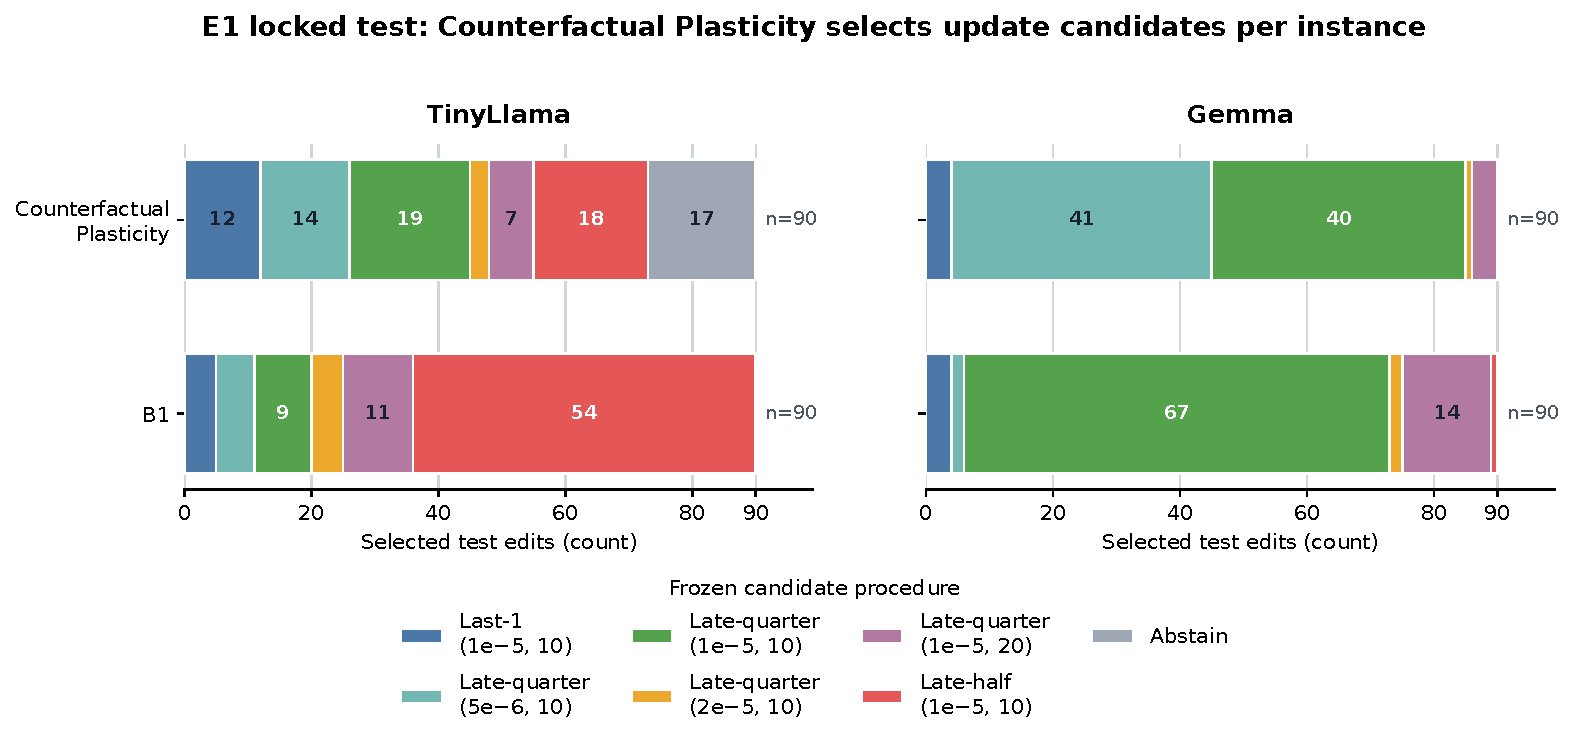
\includegraphics[width=\textwidth]{paper2_e1_selection_distributions.pdf}
    \caption{\textbf{Locked E1 candidate-selection distributions.} CP uses all
    six candidates on TinyLlama with 17 abstentions and five of six on Gemma
    with no abstention.}
    \label{fig:e1_selection_distributions}
\end{figure*}

\paragraph{Forecasting diagnostics.}
On E1 test candidates, gain MAE is 0.134 for TinyLlama and 0.160 for Gemma,
with $R^2=0.994$ and $0.992$. Damage MAE is 0.094 and 1.882, with $R^2=0.485$
and $0.656$. Candidate-level $\sigma_D$ correlates with absolute damage error
at $\rho=0.557$ ($p=2.25\times10^{-45}$) for TinyLlama and $\rho=0.459$
($p=1.69\times10^{-29}$) for Gemma; mean $\sigma_D$ is also larger on harmful
than non-harmful candidate outcomes. The S2 full-scope result ($\rho=0.072$)
shows that this diagnostic relation need not transfer under structural shift.

\begin{figure*}[t]
    \centering
    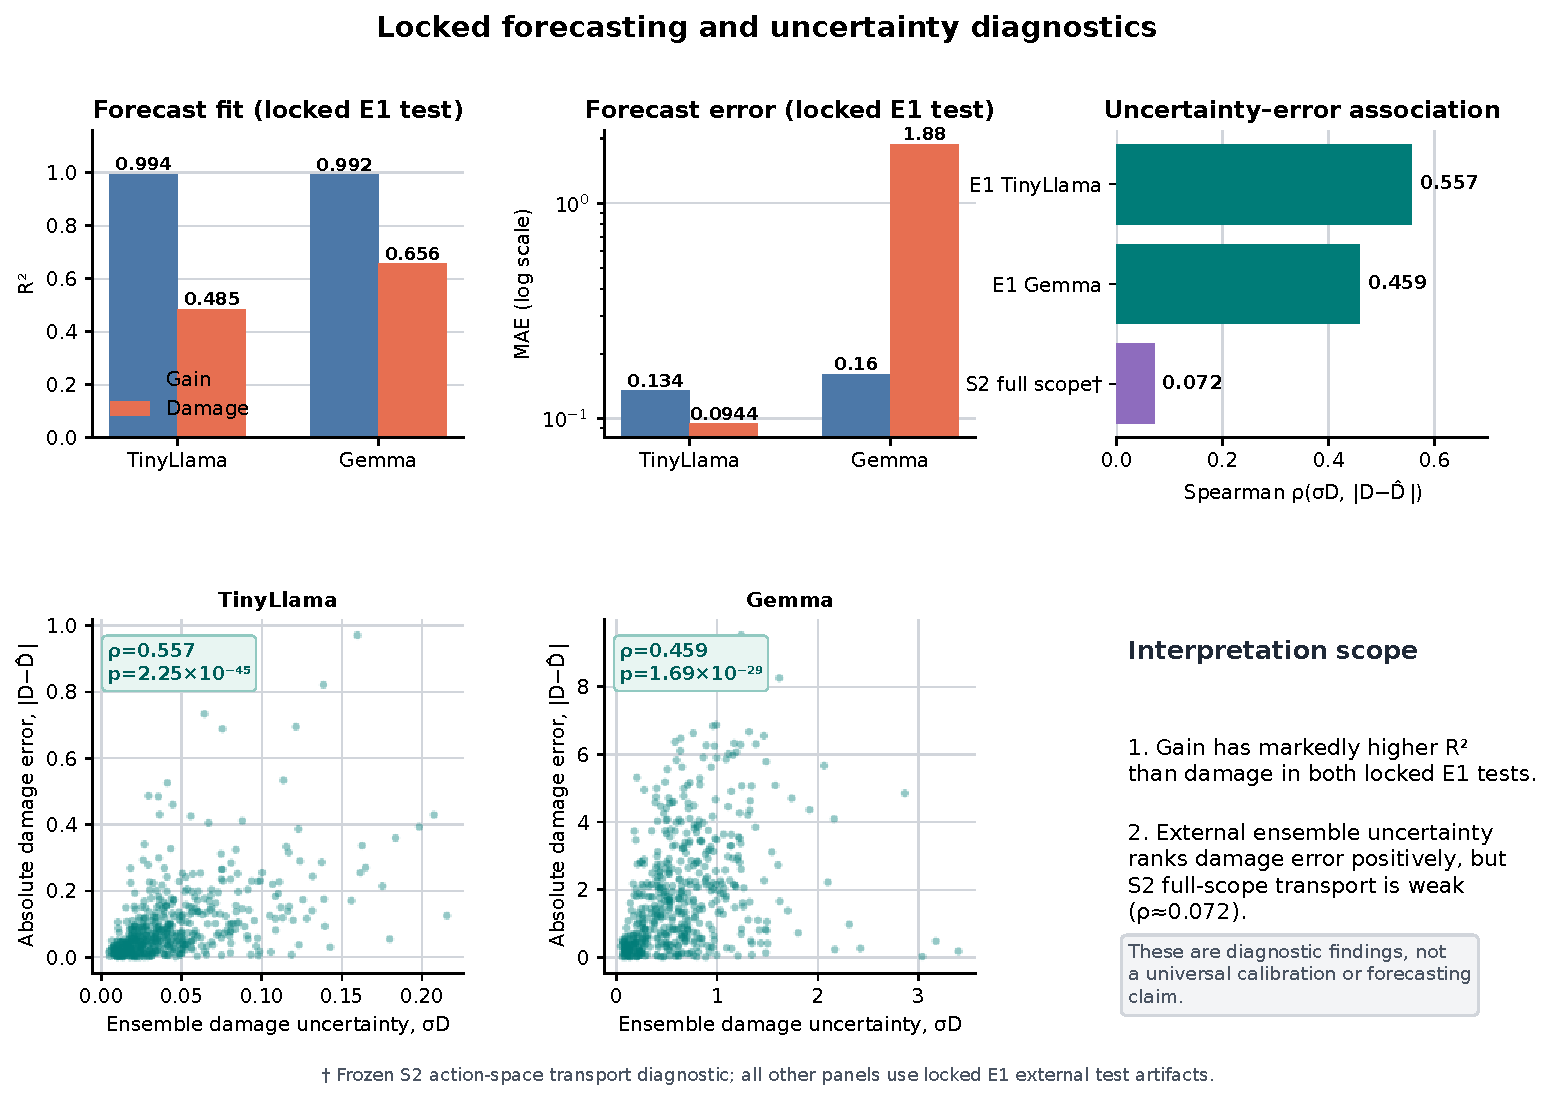
\includegraphics[width=\textwidth]{paper2_forecasting_uncertainty_diagnostics.pdf}
    \caption{\textbf{Forecasting and uncertainty diagnostics.} E1 reproduces
    the acquisition--damage predictability asymmetry and positive association
    between ensemble damage disagreement and absolute damage error, while the
    S2 full-scope transport regime shows a near-collapse of this association.}
    \label{fig:forecast_uncertainty}
\end{figure*}

\paragraph{Frozen hypotheses.}
H1 (lower harmful-decision rate than B1 in the same six-candidate space) is
supported on both models. For H2, the observed behavior satisfies its intended
qualitative content---positive useful acquisition without collapse to a single
candidate or universal abstention---but we avoid a binary claim absent an
explicit frozen quantitative threshold. H3, the descriptive positive
association between candidate-level damage uncertainty and absolute damage
error, is supported on both models and is not itself a risk-control guarantee.

\bibliography{iclr2027_conference}
\bibliographystyle{iclr2027_conference}


\end{document}
